
\documentclass[12pt,letterpaper]{article}


\usepackage[top=1in, 
		    bottom=1in,
		    left=1in,
		    right=1in]{geometry}
\usepackage{setspace}	% makes the \singlespacing, \onehalfspacing, and \doublespacing commands available
% \usepackage[en-US]{datetime2}
% \DTMlangsetup{showdayofmonth=false}
% \usepackage{titlesec}
\usepackage{listings}	% allows for placing programming code to be displayed correctly
\usepackage{siunitx}	% units
\usepackage{amsmath}
\usepackage{amsfonts}
\usepackage{amssymb}
\usepackage{graphicx}
\usepackage{booktabs}
\usepackage{multirow}
\usepackage{pgfplots}
\pgfplotsset{compat=newest}
\usepackage{tikz}
%\usetikzlibrary{shapes.geometric}
% \usepgfplotslibrary{external} 
% \tikzexternalize[prefix=pdfimages/,
% 		        mode=list and make]
\usepackage{caption}
\usepackage[list=true,
		     listformat=simple]{subcaption}
%\usepackage{cleveref}	% this should really go last
% \usepackage[colorlinks,
% 		     linkcolor=black,
% 		     citecolor=black,
% 		     plainpages=false,
% 		     pdfpagelabels]{hyperref}
% \usepackage[all]{hypcap}
\usepackage{cleveref}
% \doublespacing

\pagenumbering{gobble}
\newcommand{\mymder}[2]{\ensuremath{\frac{\mathrm{D}#1}{\mathrm{D}#2}}}
\newcommand{\mypder}[2]{\ensuremath{\frac{\partial #1}{\partial #2}}}
\newcommand{\mypdertwo}[2]{\ensuremath{\frac{\partial^2 #1}{\partial #2^2}}}
\newcommand{\mymdervec}[1]{\ensuremath{mypder{#1}{t} + }}
\newcommand{\myder}[2]{\ensuremath{\frac{d#1}{d#2}}}
\newcommand{\mydiv}[1]{\ensuremath{\nabla \cdot {#1}}}
\newcommand{\myfrac}[2]{\ensuremath{^{#1}\!/_{#2}}}
\newcommand{\myfunc}[2]{\ensuremath{#1 \left( #2 \right)}}
\newcommand{\myparen}[1]{\ensuremath{\left( #1 \right)}}
\newcommand{\mybrack}[1]{\ensuremath{\left[ #1 \right]}}
\newcommand{\mybrace}[1]{\ensuremath{\left\{ #1 \right\}}}
\newcommand{\mysin}[1]{\ensuremath{\myfunc{\mathrm{sin}}{#1}}}
\newcommand{\mycos}[1]{\ensuremath{\myfunc{\mathrm{cos}}{#1}}}
\newcommand{\myexp}[1]{\ensuremath{\myfunc{\mathrm{exp}}{#1}}}
\newcommand{\myint}[4]{\ensuremath{\int_{#1}^{#2} {#3} d {#4}}}


\newcommand{\Rld}{\ensuremath{\mathit{Re}}}
\newcommand{\St}{\ensuremath{\mathit{St}}}
\newcommand{\Prn}{\ensuremath{\mathit{Pr}}}
\newcommand{\Sc}{\ensuremath{\mathit{Sc}}}
\newcommand{\Sh}{\ensuremath{\mathit{Sh}}}
\newcommand{\Nu}{\ensuremath{\mathit{Nu}}}
\newcommand{\Bi}{\ensuremath{\mathit{Bi}}}


\let\textacute\'
\let\textgrave\`


\newcommand{\includetikz}[2]{%
    \tikzsetnextfilename{#2}%
    \input{#1#2.tex}%
}

\begin{document}

\noindent
MECH 131A Homework 3

\noindent
Assigned date: October $19^{\mathrm{th}}$, 2024

\noindent
Due date: October $25^{\mathrm{th}}$, 2024

\subsubsection*{Instructions}
\begin{enumerate}
	\item Indicate the names of your study group members.
	\item Draw a sketch of the problem.
	\item If using a specific solution methodology is specified, please include a copy of the Python/MATLAB script.
	\item If using a specific solution methodology is \textit{not} specified, please include a copy of your computational methodology.
\end{enumerate}


\subsubsection*{Problem Set}
\begin{enumerate}

    \item Consider a plane composite wall that is composed of two materials of thermal conductivities $k_A = \SI{0.1}{\watt\per\meter\per\kelvin}$ and $k_B = \SI{0.04}{\watt\per\meter\per\kelvin}$ and thicknesses $L_A = \SI{10}{\milli\meter}$ and $L_B = \SI{20}{\milli\meter}$.
    The contact resistance at the interface between the two materials is known to be \SI{0.30}{\square\meter\kelvin\per\watt}.
    Material A adjoins a fluid at \SI{200}{\celsius} for which $h = \SI{10}{\watt\per\square\meter}$, and material B adjoins a fluid at \SI{40}{\celsius} for which $h = \SI{20}{\watt\per\square\meter}$.
    
    \begin{enumerate}
        \item What is the rate of heat transfer through a wall that is \SI{2}{\meter} high by \SI{2.5}{\meter} wide?
        \item Sketch the temperature distribution.
        \item Assume material B is exposed to air at \SI{40}{\celsius} moving at \SI{10}{\meter\per\second}.
        Redo parts (a) and (b) using the average heat transfer coefficient.
    \end{enumerate}

    \item For each of the following cases, determine an appropriate characteristic length $L_c$ and the corresponding Biot number $\Bi$ that is associated with the transient thermal response of the solid object.
    State whether the lumped capacitance approximation is valid.
    If temperature information is not provided, evaluate properties at $T = \SI{300}{\kelvin}$.
    Refer to the figure.
    \begin{enumerate}
        \item A toroidal shape of diameter $D = \SI{50}{\milli\meter}$ and cross-sectional area $A_c = \SI{5}{\square\milli\meter}$ is of thermal conductivity $k = \SI{2.3}{\watt\per\meter\per\kelvin}$.
        The surface of the torus is exposed to a coolant corresponding to a convection coefficient of $h = \SI{50}{\watt\per\square\meter\per\kelvin}$.
        
        \item A long, hot AISI 304 stainless steel bar of rectangular cross section has dimensions $w = \SI{3}{\milli\meter}$, $W = \SI{5}{\milli\meter}$, and $L = \SI{100}{\milli\meter}$.
        The bar is subjected to a coolant that provides a heat transfer coefficient of $h = \SI{15}{\watt\per\square\meter\per\kelvin}$ at all exposed surfaces.
        
        \item A long extruded aluminum (Alloy 2024) tube of inner and outer dimensions $w = \SI{20}{\milli\meter}$, $W = \SI{24}{\milli\meter}$, respectively, is suddenly submerged in water, resulting in a convection coefficient of $h = \SI{37}{\watt\per\square\meter\per\kelvin}$ at the four exterior tube surfaces.
        The tube is plugged at both ends, trapping stagnant air inside the tube.
        
        \item An $L = \SI{300}{\milli\meter}$ long solid stainless steel rod of diameter $D = \SI{13}{\milli\meter}$ and mass $M = \SI{0.328}{\kilogram}$ is exposed to a convection coefficient of $h = \SI{30}{\watt\per\square\meter\per\kelvin}$.
        
        \item A solid sphere of diameter $D = \SI{12}{\milli\meter}$ and thermal conductivity $k = \SI{120}{\watt\per\meter\per\kelvin}$ is suspended in a large vacuum oven with internal wall temperatures of $T_{\mathit{sur}} = \SI{20}{\celsius}$.
        The initial sphere temperature is $T_i = \SI{100}{\celsius}$, and its emissivity is $\epsilon = 0.73$.
    \end{enumerate}

    \begin{figure}[!htpb]
        \centering
        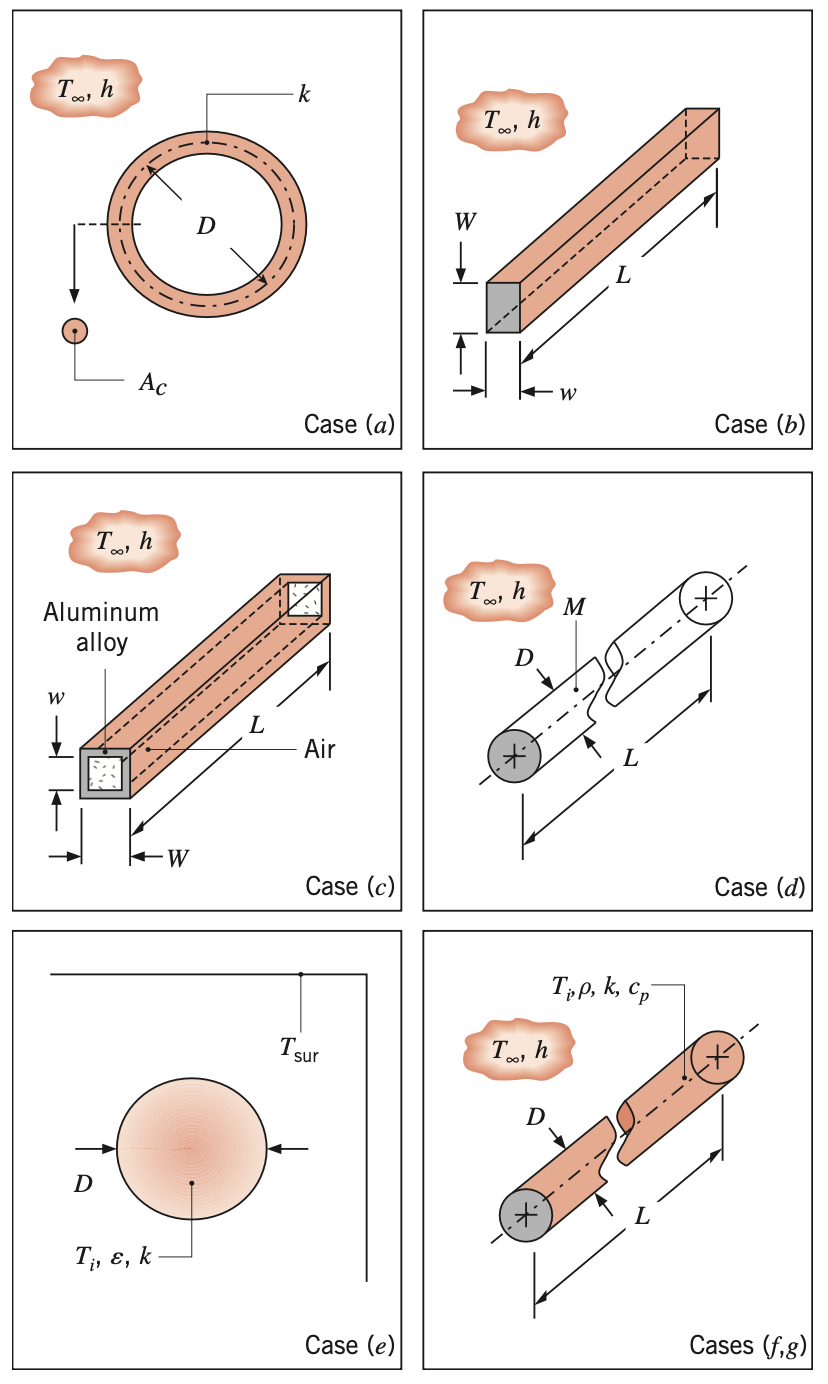
\includegraphics[width=0.75\linewidth]{./image1.png}
    \end{figure}

    \item Before being injected into a furnace, pulverized coal is preheated by passing it through a cylindrical tube whose surface is maintained at $T_{\mathrm{sur}} = \SI{1000}{\celsius}$.
    The coal pellets are suspended in an airflow and are known to move with a speed of \SI{3}{\meter\per\second}.
       If the pellets may be approximated as spheres of 1-mm diameter and it may be assumed that they are heated by radiation transfer from the tube surface, how long must the tube be to heat coal entering at \SI{25}{\celsius} to a temperature of \SI{600}{\celsius}?
        Is the use of the lumped capacitance method justified?
        
        \item Stainless steel (AISI 304) ball bearings, which have uniformly been heated to \SI{850}{\celsius}, are hardened by quenching them in an oil bath that is maintained at \SI{40}{\celsius}.
        The ball diameter is \SI{20}{\milli\meter}, and the convection coefficient associated with the oil bath is \SI{1000}{\watt\per\square\meter\per\kelvin}.
        \begin{enumerate}
        		\item Compare the initial heat transfer and temperature change to the long-term heat transfer and temperature change on plot with non-demensional time as $x$-axis.
		Indicate the range on the graph when each asymptotic approximation is applicable.
		\item Plot the temperature heat transfer profiles using both planar and spherical models and comment on the similarities and differences. 
        		\item If quenching is to occur until the surface temperature of the balls reaches \SI{100}{\celsius}, how long must the balls be kept in the oil? What is the center temperature at the conclusion of the cooling period?
		\item If \num{10000} balls are to be quenched per hour, what is the rate at which energy must be removed by the oil bath cooling system in order to maintain its temperature at \SI{40}{\celsius}?
	\end{enumerate}

%    \item Consider the velocity boundary layer profile for flow over a flat plate to be of the form $u = c_1 + c_2 y$.
%    Applying appropriate boundary conditions, obtain an expression for the velocity profile in terms of the boundary layer thickness $\delta$ and the free stream velocity $u_\infty$.
%    Using the integral form of the boundary layer momentum equation, obtain expressions for the boundary layer thickness and the local friction coefficient, expressing your result in terms of the local Reynolds number.
%    Present your results to seven significant figures.
%    Compare your results with those obtained from the exact solution and the integral solution with a cubic profile.

    \item Recreate the table giving the solution for boundary layer equation given in terms of the similarity variable, $\eta = y \sqrt{u_\infty / \nu x}$, for $f$, $f'$, and $f''$ to six significant digits.

    \item Using the results from the previous problem, verify the textbook's claim that the local skin friction coefficient is given by

    \begin{equation*}
        C_f = 0.664 \mathit{Re}^{1 / 2}.
    \end{equation*}

    Verify this relationship by integrating the boundary layer equation given in terms of the similarity variable, $\eta = y \sqrt{u_\infty / \nu x}$.
    Give your answer to six significant figures.
    
    \item Mercury, ethylene glycol, and water flow over a flat plate at the same Reynolds number at \SI{300}{\kelvin}.
    Comment on the relative velocities of the flows, the relative sizes of the thermal and momentum boundary layers, the relative sizes of the Nusselt numbers, and relative sizes of the heat transfer coefficient as the flow moves down the plate.
    Provide sketches for the last three items in the previous sentence.

\end{enumerate}


\end{document}
